\chapter{Generating Art with Computers}
\label{ch:art-computers}

This book has explored the deep connection between logic
and computing, especially how equations can be used to 
write computer programs. In this last chapter, we're going 
to turn our attention to acts of creativity. Can logic and
equations really be used to create works of art?

\section{Representing Images in a Computer}

Before we can create art on a computer, we need some way of
\emph{storing} art on the computer. So how does a computer 
store a picture?

The answer, it turns out, is surprisingly pedestrian. Ignoring
color for now, you can think of computer displays, like the
screen on your computer or phone, as many tiny dots that are
arranged in a rectangular grid of $M$ rows and $N$ columns.
Each one of those tiny dots is called a \emph{pixel}, which
at one time was short-hand for ``picture element.''
For example, the computer we are using right now has 900 rows
and 1440 columns, and that's usually described as a 
$1440\times900$ display. Again, ignoring color, each pixel can
be either on or off, so to describe a picture in a computer,
we simply need to specify which pixels are on and which ones
are off. The simplest way to do this is to have a list of
numbers, where each number corresponds to a pixel. Even better,
we can use a list of rows, each of which has a number for each
pixel in the row. Figure~\ref{fig:glider-in-images} illustrates 
this process for a $4\times4$ image. As you can see, the pixel
in row $i$ and column $j$ is on precisely when the $j^\text{th}$
entry in the $i^\text{th}$ list is a 1.

\begin{figure}
\begin{center}
\begin{minipage}{3cm}
\begin{verbatim}
'((0 1 0 0) 
  (0 0 1 0) 
  (1 1 1 0) 
  (0 0 0 0))
\end{verbatim}
\end{minipage}%
\begin{minipage}{3cm}
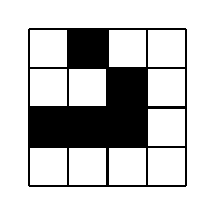
\begin{tikzpicture}[thick, scale=0.5]
\draw (0,0) grid (4,4);
\foreach \c in {(0,1), (1,1), (2,1), (2,2), (1,3)}
    \fill \c + (1, 1) rectangle \c;
\end{tikzpicture}
\end{minipage}
\end{center}
\caption{A Picture Encoded as a List of Lists of Pixels}
\label{fig:glider-in-images}
\end{figure}

It may not seem like it, but using lists to represent images is
a tremendous step. We started this book talking about the boundary
or interface between software and hardware, and this boundary is
perfectly illustrated by this representation of images. Pictures
are mysterious, but lists aren't. From the software perspective,
generating an image is nothing more than generating a list of
numbers, and generating lists is precisely the sort of thing that
we've been using equations for throughout this book. So everything
that you've learned is directly applicable. It is up to the hardware 
to interpret the list of numbers as an image and display it in
that way. 

Solutions like this are commonplace in computer science,
where complex problems are solved by splitting the problem into 
different \emph{layers}, where each layer provides an abstraction 
to the layer above. In our case, the hardware layer provides the
illusion, or abstraction, that images are really nothing more than
lists of numbers, and the software creates ``images'' by constructing
simple lists---a much more manageable task. In more complex systems,
there can be dozens of such layers.

All that is well and good, but what color? The human eye perceives
color using specialized cells, called \emph{cones}, in the central
part of the retina. There are three types of cones, each one sensitive
to a different range of colors. There is some overlap in the range
of colors that each type of cone can detect, but it is mostly accurate
to think in terms of cones that are sensitive to shades of red, green, 
and blue. 

So the way to build color images is to let each pixel be on or off in
each of the different colors. For example, the first row from 
Figure \ref{fig:glider-in-images} looks like this for a black-and-white
image:
\begin{itemize}
    \item \textsf{(0 1 0 0)}
\end{itemize}
But in color, we may have a red pixel like this:
\begin{itemize}
    \item \textsf{((0 0 0) (1 0 0) (0 0 0) (0 0 0))}
\end{itemize}
Here we follow the common convention that colors are specified in triples, 
and with the order red-green-blue, so that \textsf{(1 0 0)} is pure red.
This allows us to have eight separate colors, including black, white, red,
green, and blue, and combinations of red, green, and blue, resulting
in cyan, magenta, and yellow. That's better, but not a lot of colors.

To get more colors, we need to allow more subtle \emph{blending} of the
colors red, green, and blue. For example, a pixel with both red and green
on but not blue results in yellow. If you allow a pixel to have intensity
of color, then you can also represents shades of red and green, resulting
for example in orange. The human eye can detect more than 256 shades of
each color, but experience suggests that 256 shades are enough to produce
realistic color. So it is common to specify shades of red as a number from
0 to 255. Using this scheme, the list \textsf{(255 140 0)} can be used to
describe a dark shade of orange.

In principle, that's all we need to create images, even colorful images.
However, this is where additional layers, between the software and hardware
layers, can be helpful. Imagine, for example, a function called \textsf{draw-line}
that adds a line to an image. This would keep you from having to decide
which pixels are on the path of the line and need to be set to the right
color in the image.

The definition of \textsf{draw-line} requires a little care. In some
computer languages, it makes sense to speak of ``adding a line to an image,''
but that does not make sense when using equations to define functions, because
functions always return the same value for the same inputs---they do not change
their inputs. So the \textsf{draw-line} function may actually look like this
\begin{itemize}
    \item \textsf{(draw-line image x1 y1 x2 y2 color)}
\end{itemize}
Here \textsf{image} is an array of pixel values, the xs and ys are the
coordinates, and the \textsf{color} is the color of the line.
What the function returns is a new image that consists of a line from the 
start point to the end point on top of the original image.

\begin{aside}
The process of drawing a line from one point to another is actually quite
tricky. One problem is that there are many subtle cases to consider, and
if you don't take care of these cases correctly, the result does not look
like a line at all. For example, suppose the start point is $(1,1)$ and
the end point is $(10,10)$ then the line consists of the points $(2,2)$,
$(3,3)$, and so on. All you have to do is find the right $y$ value for
each $x$. No problems there. But if the end point is $(2,10)$ instead,
then simply finding the ``right'' $y$ for each $x$ will not work. Instead
of a line, you would end up with just two widely separated points. This
is an extreme case, but similar issues will show up when drawing many 
different lines.

Another problem concerns speed. In typical graphics applications, the
computer needs to draw millions, even billions, of lines per second.
The computer scientist Jack Bresenham developed an algorithm in the
1960s to solve this particular problem. Improved versions of this 
algorithm are still in use today.
\end{aside}

We're sure you can think of many more useful functions similar to 
\textsf{draw-line}. Some of these may be functions that draw
other shapes, like triangles, squares, rectangles, polygons, circles, 
ellipses, and so on. The important thing to realize is that all of
these functions work on images represented as lists of pixel colors. 
What this achieves, really, is to add a layer that understands
basic geometric shapes on top of the layer that represents an image 
as a list of pixel colors.

There is another, very different, layer that can be defined
on top of the list of pixel colors. Instead of functions that can
create new graphical objects, we can write functions that change the
image in other ways. For example, suppose that an image has a
very dark line on top of a bright background. This creates a very 
sharp boundary between the line and the background, but it can be
smoothed by averaging the colors of a pixel and its neighbors. The
bright pixels on one side of the boundary become a little darker,
and the dark pixels on the other side become a little lighter, 
resulting in a more subtle boundary. This is the basic idea behind
functions such as \textsf{blur} that manipulate images at the level
of individual pixels and their neighbors. Such functions are usually
called \emph{image filters}, and they are very popular in image
processing software. These filters are yet another layer that can be 
used to create images in a computer, either with or without other
layers, such as the one that creates geometric shapes.

\section{Generating Images Randomly}

One way to generate more artistic images is to insert a layer of
randomness on top of the layers that create geometric objects. 
When an artists paints on canvas, she may be layering paints on
with a brush that has a certain texture, and her strokes will create
a complex pattern that is more than just a line.
Figure~\ref{fig:line-art} shows how this may happen in code. One
image shows a straight line from the point $(0,0)$ to $(14,14)$, 
and the other shows how a more artistic line may be rendered by 
proceeding from the point $(0,0)$ to $(14,14)$ in a sequence of
directed and yet random steps. You can also so the same with other
geometric shapes, as in noisy rectangles, and circles that are
mostly, but not exactly round.

\begin{figure}
\begin{center}
\begin{tabular}{ll}
\includegraphics[scale=0.3]{images/straight-line.png} &
\includegraphics[scale=0.3]{images/random-line-art.png} \\
\end{tabular}
\end{center}
\caption{Straight Line vs.~a Line Made Up of Random Segments}
\label{fig:line-art}
\end{figure}

But what do we mean by random? Nothing in a computer is truly random,
and definitely nothing can be random when it's computed using 
equations, as we have been in this book. But consider this sequence:
$$0, 1, 5, 3, 4, 8, 6, 7, 2, 0$$
This sequence looks fairly random, doesn't it? In fact, it is anything
but! It results from executing the following function:
\begin{Verbatim}
(defun f (n)
 (if (zp n)
     0
     (mod (+ (* 4 (f (- n 1))) 1) 9)))
\end{Verbatim}
As you can easily check, \textsf{(f 0)} is equal to 0, \textsf{(f 1)} 
is equal to 1, \textsf{(f 2)} is equal to 5, \textsf{(f 3)} is equal
to 3, and so on. So what we have is a function whose outputs appear
to be random, but are in fact deterministic (as is the case with all 
functions). We say that these functions are \emph{pseudo-random}, and 
this is the way that we can introduce as aspect of randomness into our
pictures.

The function \textsf{f} above belongs to a family of pseudo-random
functions. Each of these functions has a \emph{seed} value, which is
what it returns for input $0$. It also has a \emph{multiplier} and an \emph{increment},
which are used to scale and add to the result of the previous random
number---in our case, the multiplier was $4$ and the increment $1$.
Finally, these functions feature a \emph{modulus} used to keep the
random numbers in a given range, in our case $9$. 

It is common to write pseudo-random functions line \textsf{f} such 
that the argument is its previous value. This simply avoids the need 
to use recursion to find the previous values of \textsf{f} and is much 
faster. When the function is written in this way, we can think of calling
it with the current seed, and the function returns the next random number.
The next time the function is called, it should be called with the new
seed value, which is just the previous random number the function returned.
Here is how we could write a pseudo-random \textsf{g} that returns the
same values as \textsf{f}, but with this approach of passing the seed
value as the argument.
\begin{Verbatim}
(defun g (seed)
  (mod (+ (* 4 seed) 1) 9))
\end{Verbatim}

One more thing. The functions \textsf{f} and \textsf{g} always return
a natural number between 0 and 8. All functions that generate pseudo-random
numbers using this strategy have a similar property, since they must return
a natural number between 0 and $M-1$, where $M$ is the modulus. It is
often convenient to work with rational random numbers between $0$ and $1$
instead of working with integers, and all of our pseudo-random functions
can do this simply by dividing the final result by $M$. We will assume
that we are using such rational pseudo-random functions from now on.

So let's take it for granted that we have a pseudo-random function 
called \textsf{random}, and let's use to make more seemingly creative 
shapes. For example, we can use to generate jagged lines
like this:
\begin{Verbatim}
(defun jagged-line (image x1 y1 x2 y2 seed)
 (if (< x1 x2)
     (let* ((rand (random seed))
            (offset (- rand 1/2))
            (slope (/ (- y2 y1) (- x2 x1)))
            (next-x (+ x1 1))
            (next-y (+ y1 slope offset)))
       (jagged-line (draw-line image x1 y1 next-x next-y 'black)
                    next-x next-y x2 y2 rand))
     image))
\end{Verbatim}
This function draws a jagged line from $(x1,y1)$ to $(x2,y2)$ by
drawing line segments spaced 1 unit apart in the $x$ direction. 
The $y$ coordinate of each segment is generally in the direction
or the slope of the straight line to $(x2,y2)$, but is offset 
by a given amount.  The function \textsf{random} returns a number 
between 0 and 1, so the \textsf{offset} is between $-1/2$ and $+1/2$.
That's not a lot, but it's enough to make the path more organic
than a straight line. This is exactly the idea behind the line
in Figure~\ref{fig:line-art}. Finally, notice how in the inductive
call to \textsf{jagged-line} the value of \textsf{seed} has been
replaced by \textsf{rand}, which is precisely the last value returned
by \textsf{random}.

\section{Generating Purposeful Images}

Random images can be very nice, but are they really art? Can a computer
program produce real works of art? That question may be unanswerable.
If you believe that only human beings can ever be creative, then any
work produced by a program simply cannot be considered art, by
definition. But however you feel about this question, there are a
handful of programs that could reasonably be called artists. Let's
look at one of these.

Written over a span of decades by artist Harold Cohen, the program 
AARON was designed in part as an exploration of artmaking. Cohen's 
initial goal was to determine when a group of abstract marks can
be recognized as a coherent image. The earliest versions of AARON 
could do very little, and they knew very little about art. Young
AARON knew the difference between a figure and the ground, and also
the difference between an open figure and a closed figure, but
little more. 

What made those early versions of AARON effective was a layer that
stood on top of the low-level drawing layer. This layer was essentially
a list, but instead of pixel colors, this list contained graphical objects 
and their location. Adding a new figure to the canvas was accomplished
by adding a new object to this master list. The real breakthrough, 
though, is that this list could be examined during the process of adding
a new figure, so AARON could effectively reflect on the work it had
done before proceeding. This allowed AARON to make decisions based on
artistic principles, such as balance and proportion. This breakthrough
proved so successful that it carried over into all future versions of
AARON.

An obvious way to enhance AARON would have been to add more graphical
primitives at this point, such as new figures that it could draw. But 
the next step in AARON's evolution was something more profound. What
Cohen did was to enhance AARON so that it could ``scribble'' around
``core figures.'' This idea came from observing the way children 
scribble on paper, and in particular the key moment when the children
seemed to realize that a figure they scribbled actually represented a
real object in some world. From AARON's perspective, the main improvement
was a two-step strategy where core figures were placed in a virtual world, 
and then the picture was allowed to evolve by basically tracing a path
around them. This strategy resulted in paintings with much more complexity
and a sense of realism, in that the end product showed realistic-looking
objects that seemed to be inspired from the real world. Certainly, if a
human had drawn these shapes, there would have been no doubt that they
were reflections of the real world.

From this point on, AARON became more and more \emph{representational} in
the works it produced. This took three main sources of improvement. The first
was a database of core figures that combined to represent visually some
objects from the real world. Each core figure was represented as a list of
key points that provided essentially an outline, and the figures were connected
in space and orientation.
For example, a plant could be represented by
a trunk, some branches, and some leaves. Each of those may be a core figure,
and the figures would be related to each other geometrically, which is to say
that the branches are connected to the trunk, and the leaves to the branches.
This basic strategy worked to model even complex objects, such as a basic human
form and a recognizable image of the Statue of Liberty.

The second improvement was a series of algorithms that could create reasonable
objects made up of core figures. It is simply impractical to model all possible
objects using core figures. So Cohen wrote some algorithms that allowed AARON to
imagine plants, or as he called them \emph{quasi-plants}. It should not surprise
you that these algorithms made extensive use of pseudo-randomness. At this point,
AARON's paintings featured recognizable human shapes in an environment rich with 
flora.

Finally, the third improvement was the development of a set of rules that 
let AARON render an image from a world described by core figures. Essentially,
these rules amount to expertise in drawing. For example, the core figures occupy
a space in three dimensions, and the rules determine how AARON is to deal with
geometric problems such as perspective and occlusion. That is, figures farther
away must appear smaller in the final image, and one core figure in front may
partially hide a figure that is farther away. AARON is truly becoming an expert
painter, if not a true artist.

AARON's paintings from this time represent a high point in its work, and they
were exhibited in museums. But there was a hidden limitation, in that the core figures 
used to build AARON's model of the world were two-dimensional. The figures could be 
placed in a three-dimensional world, but the realism in AARON's work was partially
due to the limitations in the scale of it painting. Cohen intended to create larger
and more complex paintings, and he felt that this increase in scale would require a
more detailed model of the real world in AARON's data structures.

So Cohen embarked on a new modeling phase, involving more detailed and fully 
three-dimensional models of the objects that AARON would draw, such as the human
body. These models were made of groups of three-dimensional points that were
related to other similar groups, in a way that is clearly derived from the earlier
core figures. In a tradition dating back to da Vinci and Michelangelo, the models
for the human body were taken directly from anatomical studies (but thankfully in 
the modern era of AARON, this information could be found in textbooks.) This shift
created many complications, of course, in that AARON's model was now three-dimensional,
so it was forced to create the two-dimensional core images before rendering a
painting. 

The complications are significant, but they add little to our story, so we will
let the interested reader to pursue this further by finding Cohen's own description
of his work or Pamela McCorduck's very readable account of AARON's evolution as an
artist---even to the point of mixing its own pigments and painting its own artworks 
on a physical canvas. What we want to leave you with is an appreciation that 
simple principles can indeed lead to complex behavior. AARON's knowledge of the
real work is encoded as a set of points, and its expertise in drawing is encoded
as a set of rules, very much in the way we used lists and equations to write programs.
AARON is an impressive program, and it could easily be claimed that it exhibits
creativity and the right to be called an artist. But at its core, it really is 
composed of simple principles that taken as a whole happen to capture the essence of 
painting.

%%% Local Variables:
%%% mode: latex
%%% TeX-master: "book"
%%% End:
